\documentclass[12pt]{article}

\usepackage{algorithm} %pseudo-code
\usepackage{algpseudocode}
\usepackage{amsmath,amsthm,amssymb}
\usepackage{graphicx}
\usepackage{float}
\usepackage{amsmath, amssymb, amscd}
\usepackage{alltt}
\usepackage{textcomp}
\usepackage{gensymb}
\usepackage{multicol}
\usepackage{tabularx}

\newcommand{\N}{\mathcal{N}}
\newcommand{\Z}{\mathbb{Z}}
\newcommand{\R}{\mathbb{R}}
\newcommand{\bigo}{\mathcal{O}}
\newcommand{\G}{\mathcal{G}}
\newcommand{\V}{\mathcal{V}}
\newcommand{\E}{\mathcal{E}}
\newcommand{\K}{\mathcal{K}}
\newcommand{\T}{^\intercal}

\newcommand{\sups}[1]{\ensuremath{^{\textrm{#1}}}}
\newcommand{\subs}[1]{\ensuremath{_{\textrm{#1}}}}

\newcommand{\specialcell}[2][c]
{
  \begin{tabular}[#1]{@{}c@{}}#2\end{tabular}
}

\makeatletter
\newsavebox{\mybox}\newsavebox{\mysim}
\newcommand{\distras}[1]
{
  \savebox{\mybox}{\hbox{\kern3pt$\scriptstyle#1$\kern3pt}}%
  \savebox{\mysim}{\hbox{$\sim$}}%
  \mathbin{\overset{#1}{\kern\z@\resizebox{\wd\mybox}{\ht\mysim}{$\sim$}}}%
}
\makeatother
\makeatletter
\renewcommand*\env@matrix[1][c]{\hskip -\arraycolsep
  \let\@ifnextchar\new@ifnextchar
  \array{*\c@MaxMatrixCols #1}}
\makeatother
%===============================================================================
% code highlighting :
\usepackage{listings}

% define custom colors :
\usepackage{color}
\definecolor{bg}{rgb}{0.96,0.96,0.85}
\definecolor{deepblue}{rgb}{0,0,0.5}
\definecolor{deepred}{rgb}{0.6,0,0}
\definecolor{deepgreen}{rgb}{0,0.5,0}

\usepackage{xcolor}
\renewcommand{\lstlistlistingname}{Code Listings}
\renewcommand{\lstlistingname}{Code Listing}
\definecolor{gray}{gray}{0.5}
\colorlet{commentcolour}{green!50!black}

\colorlet{stringcolour}{red!60!black}
\colorlet{keywordcolour}{magenta!90!black}
\colorlet{exceptioncolour}{yellow!50!red}
\colorlet{commandcolour}{blue!60!black}
\colorlet{numpycolour}{blue!60!green}
\colorlet{literatecolour}{magenta!90!black}
\colorlet{promptcolour}{green!50!black}
\colorlet{specmethodcolour}{violet}
\colorlet{indendifiercolour}{green!70!white}

\newcommand{\framemargin}{5ex}

\newcommand{\literatecolour}{\textcolor{literatecolour}}

\newcommand\pythonstyle{\lstset{
%keepspaces=true,
language=python,
showtabs=true,
tab=,
tabsize=2,
basicstyle=\ttfamily\scriptsize,%\setstretch{.5},
stringstyle=\color{stringcolour},
showstringspaces=false,
alsoletter={1234567890},
otherkeywords={\ , \}, \{, \%, \&, \|},
keywordstyle=\color{keywordcolour}\bfseries,
emph={and,break,class,continue,def,yield,del,elif ,else,%
except,exec,finally,for,from,global,if,import,in,%
lambda,not,or,pass,print,raise,return,try,while,assert},
emphstyle=\color{blue}\bfseries,
emph={[2]True, False, None},
emphstyle=[2]\color{keywordcolour},
emph={[3]object,type,isinstance,copy,deepcopy,zip,enumerate,reversed,list,len,dict,tuple,xrange,append,execfile,real,imag,reduce,str,repr},
emphstyle=[3]\color{commandcolour},
emph={Exception,NameError,IndexError,SyntaxError,TypeError,ValueError,OverflowError,ZeroDivisionError},
emphstyle=\color{exceptioncolour}\bfseries,
%upquote=true,
morestring=[s]{"""}{"""},
morestring=[s]{'''}{'''},
commentstyle=\color{commentcolour}\slshape,
%emph={[4]1, 2, 3, 4, 5, 6, 7, 8, 9, 0},
emph={[4]ode, fsolve, sqrt, exp, sin, cos, arccos, pi,  array, norm, solve, dot, arange, , isscalar, max, sum, flatten, shape, reshape, find, any, all, abs, linspace, legend, quad, polyval,polyfit, hstack, concatenate,vstack,column_stack,empty,zeros,ones,rand,vander,grid,pcolor,eig,eigs,eigvals,svd,qr,tan,det,logspace,roll,min,mean,cumsum,cumprod,diff,vectorize,lstsq,cla,eye,xlabel,ylabel,squeeze,plot,median,std,hist},
emphstyle=[4]\color{numpycolour},
emph={[5]__init__,__add__,__mul__,__div__,__sub__,__call__,__getitem__,__setitem__,__eq__,__ne__,__nonzero__,__rmul__,__radd__,__repr__,__str__,__get__,__truediv__,__pow__,__name__,__future__,__all__},
emphstyle=[5]\color{specmethodcolour},
emph={[6]assert,range,yield},
emphstyle=[6]\color{keywordcolour}\bfseries,
% emph={[7]self},
% emphstyle=[7]\bfseries,
literate=*%
{:}{{\literatecolour:}}{1}%
{=}{{\literatecolour=}}{1}%
{-}{{\literatecolour-}}{1}%
{+}{{\literatecolour+}}{1}%
{*}{{\literatecolour*}}{1}%
{/}{{\literatecolour/}}{1}%
{!}{{\literatecolour!}}{1}%
%{(}{{\literatecolour(}}{1}%
%{)}{{\literatecolour)}}{1}%
{[}{{\literatecolour[}}{1}%
{]}{{\literatecolour]}}{1}%
{<}{{\literatecolour<}}{1}%
{>}{{\literatecolour>}}{1}%
{>>>}{{\textcolor{promptcolour}{>>>}}}{1}%
,%
breaklines=true,
breakatwhitespace= true,
%xleftmargin=\framemargin,
%xrightmargin=\framemargin,
aboveskip=1ex,
frame=trbl,
%frameround=tttt,
rulecolor=\color{black!40},
%framexleftmargin=\framemargin,
%framextopmargin=.1ex,
%framexbottommargin=.1ex,
%framexrightmargin=\framemargin,
%framexleftmargin=1mm, framextopmargin=1mm, frame=shadowbox, rulesepcolor=\color{blue},#1
%frame=tb,
backgroundcolor=\color{yellow!10}
}}

% Python environment
\lstnewenvironment{python}[1][]
{
  \pythonstyle
  \lstset{#1}
}
{}

% Python for external files
\newcommand\pythonexternal[1]
{{
  \pythonstyle
  \lstinputlisting{#1}
}}

% Python for inline
\newcommand\pythoninline[1]{{\pythonstyle\lstinline!#1!}}

% end code highlighting
%===============================================================================

\DeclareMathOperator*{\argmax}{arg\,max}

\begin{document}
\small

\title{Space Simulator - Project 02}
\author{Evan Cummings and Joshua Bartz\\
CSCI 576 - Human Computer Interaction}

\maketitle

\section*{Description}

For our project idea, we would like to develop a 3D rendered engine via Python's interface to OpenGL.  As it stands, we have a 3D particle simulation and an efficient way to calculate forces between particles and such.  From this simulation, we would first like to create a space simulator - complete with gravity between planets and other space bodies and thrusters on the spacecraft which create rotational and directional momentum.  With the addition of a rear engine and front braking thrusters, this would effectively simulate a real space craft.  

Once the thruster part of the engine has been created, it would be interesting to add a missile with the same thruster system which could seek out and destroy asteroids or other space objects which may be in the spacecraft's way.  Next, multiplayer could be developed where two opponents might chase each other through an asteroid field or planetary system by following some kind of particle trail.  

Long-term development outside of the scope of this class includes random generation of planetary systems from a series of differential equation solvers which the user will run in the background.  These simulations may take several hours to complete, but will allow the user to explore these new planetary systems with their spacecraft.  From here, it would be interesting to add the option for planetary evolution, i.e., randomly generated atmosphere, oceans, and mountain ranges.  The user may then enter the atmosphere with their spacecraft, complete with physics calculations and potential failure.  This is a major highlight of the game as it would allow the user to generate and explore an entire solar system, all with the power of their home PC.  In a sense this would be similar to entering into the computer's imagination, a completely unique experience.

\subsection*{Intended users}

The intended users of the system are:

\begin{multicols}{2}
\begin{enumerate}

  \item Anyone who enjoys flying is space.

  \item People who enjoy the experience of speed.

  \item People who enjoy competition.

  \item Anyone interested in the physics of space.

  \item People looking for a casual low-stress game.

  \item People looking for a high-stress challenge.

  \item People looking for a quick game.

  \item People who enjoy wasting an entire day playing one game because it is so good.

  \item People looking for a game they never tire of.

  \item People who enjoy watching things explode.

  \item People who wonder what it would be like to fire a rocket in space.

  \item People who are technically-minded.

  \item People who just want to have a good time.

  \item Anyone who enjoys wireframe rendered 3D games.

  \item People looking to escape from reality.

  \item People who always wanted to be a space-person when they grew up but never could.

  \item Younger people.

  \item People who do not enjoy excessive violence in a video game.

  \item Parents.

  \item People who like flashing lights and colors that dazzle the senses.

  \item People with a computer.

\end{enumerate}
\end{multicols}

\subsection*{Usability requirements}

The non-functional requirements for this game will be:

\vspace{4mm}
The game will be

\begin{multicols}{2}
\begin{enumerate}

  \item fun,

  \item relatively easy to learn,

  \item realistic,

  \item rewarding,

  \item challenging,
  
  \item artistic,
  
  \item innovative,
  
  \item visually pleasing,
  
  \item surprising,
  
  \item informative,
  
  \item educational,
  
  \item awe inspiring,
  
  \item worth paying money for,
  
  \item able to make the \emph{user} feel artistic,
  
  \item full of infinite possibilities,

  \item replayable,

  \item affordable,

  \item easily executable from an PC created within the last decade,

\end{enumerate}
\end{multicols}

\subsection*{Functional requirements}

\noindent \textbf{High priority:}

The users of the game should be able to

\begin{multicols}{2}
\begin{enumerate}

  \item navigate easily between menus and the game screen,

  \item configure the controls,

  \item pause the game and return to the main menu,

  \item fly the spaceship,

  \item rotate the spacecraft 360 degrees,

  \item move the spacecraft side to side,

  \item change the speed of the spacecraft in all directions, 

  \item control the thrust of the main engine,

  \item visually see their current speed and acceleration,

  \item control the craft with a mouse and keyboard,

  \item choose from a menu to start or stop a game or configure settings,

\end{enumerate}
\end{multicols}

\noindent \textbf{Medium priority:}

The users of the game should be able to

\begin{multicols}{2}
\begin{enumerate}

  \item avoid the gravitational pull of planets and asteroids, 

  \item have a map and a way to navigate,

  \item aim by moving a targeting reticule,

  \item know their distance from their selected destination,

  \item control the craft with a joystick,

  \item adjust the sensitivities of the mouse or joystick,

  \item invert either axis of input for the mouse or joystick,

  \item fly through a nebula and see color changes related to velocity,

\end{enumerate}
\end{multicols}

\noindent \textbf{Low priority:}

The users of the game should be able to

\begin{multicols}{2}
\begin{enumerate}

  \item dodge space debris,

  \item see on-screen vectors for moving objects,

  \item fly through rings that guide the ship into orbit of a planet,

  \item scale the game's complexity to increase the framerate of the game,

  \item display the framerate of the game,

  \item choose from several different spaceships with different attributes,

  \item customize their own spacecraft from attributes, i.e., speed, maneuverability, or color,

  \item select from a list of rendering effects to increase framerate,

\end{enumerate}
\end{multicols}

\section*{Design critique 1 feedback}

\subsection*{Evan's feedback:}

\begin{itemize}
  \item \emph{Provide a goal other than simply flying around in space.}
        
        \textbf{Decision : } \parbox[t]{5in}{We plan on implementing an obstacle course and entering into orbit around a planet.  We will also be able to launch missiles at space debris and learn about space and physics.  Also, the challenge with the simulator lies in simply avoiding collisions with planets and other space debris.}

  \item \emph{Include a clear navigation system.}
        
        \textbf{Decision : } \parbox[t]{5in}{We will indicate the current speed, direction, and acceleration of the spacecraft in a corner of the screen, as well as a compass.  Also, tiny particles will be included to give the player a sense of speed as they move through empty space.}

  \item \emph{Show the player statistics of the space vehicle such as speed.}
        
        \textbf{Decision : } \parbox[t]{5in}{New statistics and feedback options need to be explored.}

  \item \emph{Provide player customizations for the spacecraft.}
        
        \textbf{Decision : } \parbox[t]{5in}{We would like to allow the user to apply attributes to the craft such as maximum speed and maneuverability.}

  \item \emph{Make it possible to scale the difficulty and realism.}
        
        \textbf{Decision : } \parbox[t]{5in}{We would like to scale the size of the space to render and quality of visual effects, as well as a `simulator' mode providing the most realistic space movement and `arcade' mode with simplified controls.}

  \item \emph{Explicitly educate the players on the physics of space.}
        
        \textbf{Decision : } \parbox[t]{5in}{Ideas for this include Nebula color changes to particles as they gain kinetic and potential energy with a colorbar which indicates current energy in Joules.  Also, we would like to show the player a path which places the spacecraft in orbit around a planet or star.  This will include a visual indicator of direction and speed.}

  \item \emph{Challenge the player to put their spacecraft into orbit around a planet.}
        
        \textbf{Decision : } \parbox[t]{5in}{Rings may be included which the player could use to guide the spacecraft through while increasing or decreasing speed in order to obtain a stable orbit.}

  \item \emph{Model the known solar system.}
        
        \textbf{Decision : } \parbox[t]{5in}{In the time scales relevant to our game, this may be a challenge.  We have discussed increasing time and providing near- or at-light speed travel.  The physics of the planets may also be included in this simulation with gravitational forces acting between each planet and the spacecraft.}

  \item \emph{Allow the user to launch probes into space to investigate other systems.}
        
        \textbf{Decision : } \parbox[t]{5in}{While an interesting idea, the expanse of space would be difficult to model within the course of the class, but if there was an efficient way to randomly generate these other systems, this is an interesting option.}

  \item \emph{Provide a ``missile cam'' to guide missiles through obstacles.}
        
        \textbf{Decision : } \parbox[t]{5in}{Totally cool -- If we have time, this will be included.}
\end{itemize}

\subsection*{Josh's feedback:}

\section*{Menus}

The menu system has been adapted from Josh's design crit one and uses a common video game configuration with buttons accessed with the mouse or joystick.  An explanation of the individual screens are presented below.

\subsection*{Menu storyboards}

\begin{figure}[H]
  \centering
  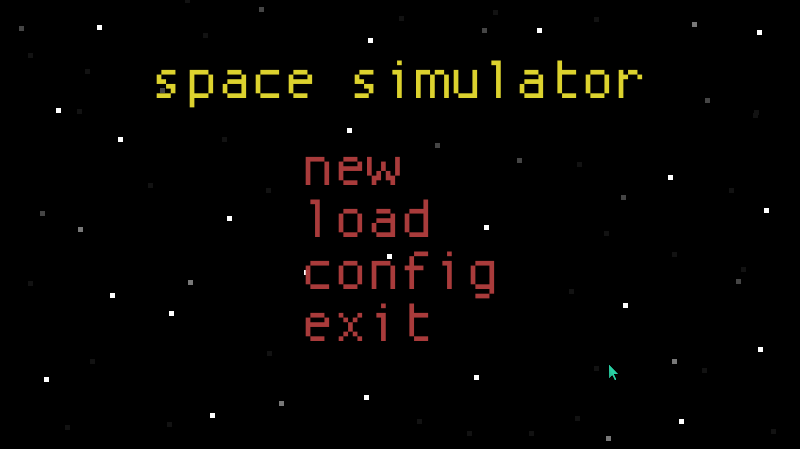
\includegraphics[scale=0.5]{../images/01-start.png}
  \caption{Start screen upon initialization.  From here the player may either start a new game, load an existing game, edit the configuration of the game, or exit.}
\end{figure}

\begin{figure}[H]
  \centering
  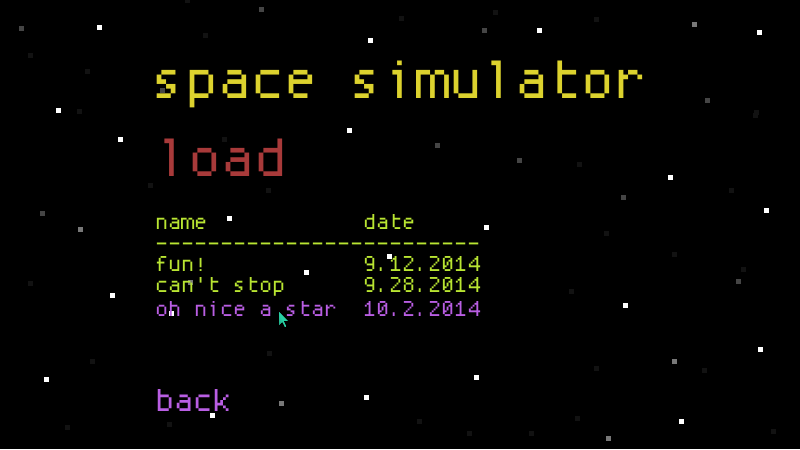
\includegraphics[scale=0.5]{../images/02-load.png}
  \caption{Load screen enabling a player to load a previously-saved game.}
\end{figure}

\begin{figure}[H]
  \centering
  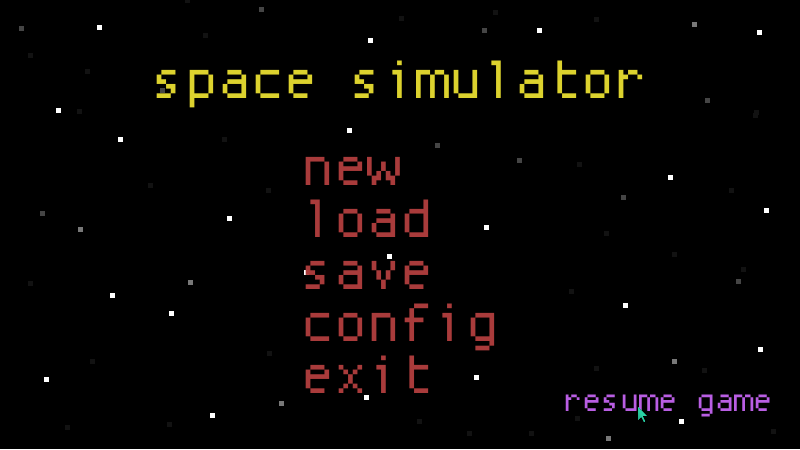
\includegraphics[scale=0.5]{../images/03-pause.png}
  \caption{Pause screen accessed at any time by pressing the ``esc'' key.}
\end{figure}

\begin{figure}[H]
  \centering
  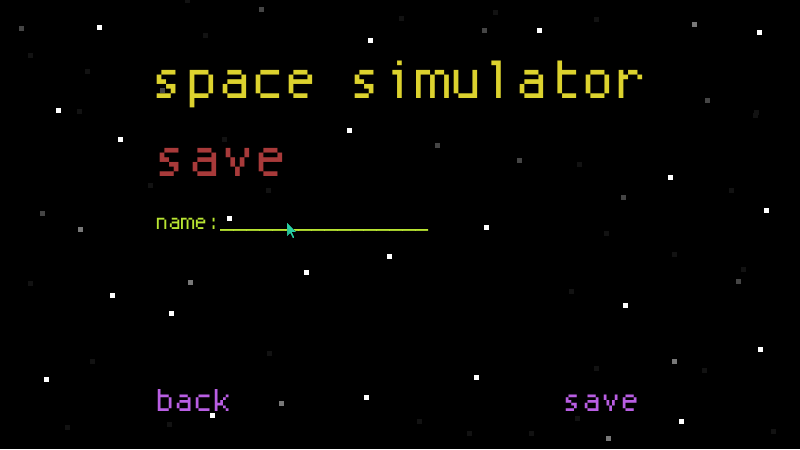
\includegraphics[scale=0.5]{../images/04-save.png}
  \caption{Save screen.  The player can name the save game and press ``save'' to save.}
\end{figure}

\begin{figure}[H]
  \centering
  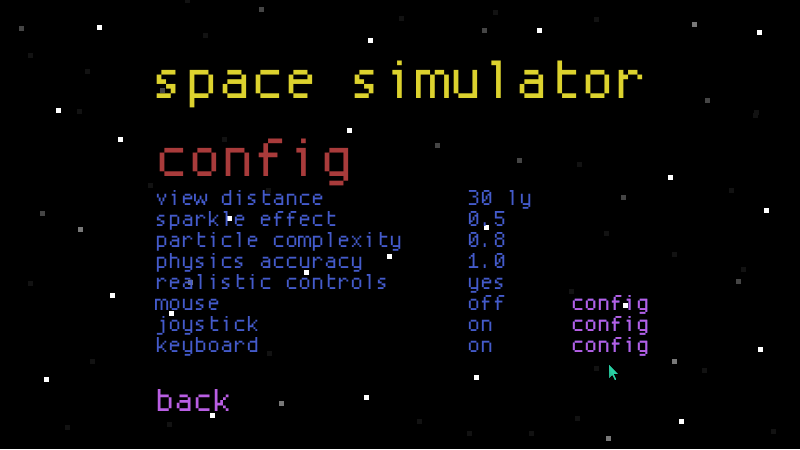
\includegraphics[scale=0.5]{../images/05-config.png}
  \caption{Config for global settings with access to control config screens.  The player clicks on the parameter which increments the setting.  Once any setting has been changed, nothing more is required of the player.}
\end{figure}

\begin{figure}[H]
  \centering
  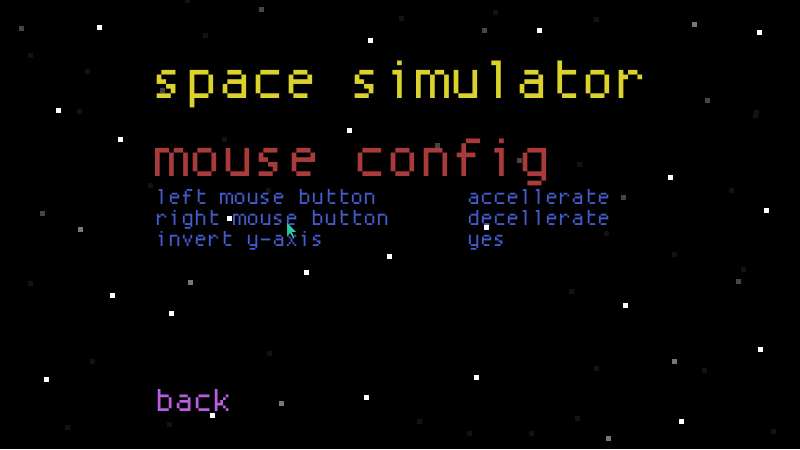
\includegraphics[scale=0.5]{../images/06-mouse_config.png}
  \caption{Mouse config, the user may select from a list of logical actions for both left and right buttons.}
\end{figure}

\begin{figure}[H]
  \centering
  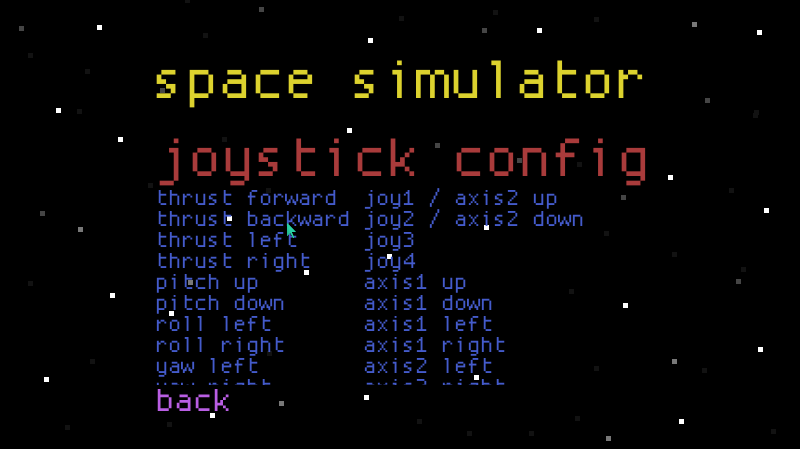
\includegraphics[scale=0.5]{../images/07-joystick_config.png}
  \caption{Joystick config.  User may set the button by pressing the desired joystick button or moving the joystick in a particular direction.}
\end{figure}

\begin{figure}[H]
  \centering
  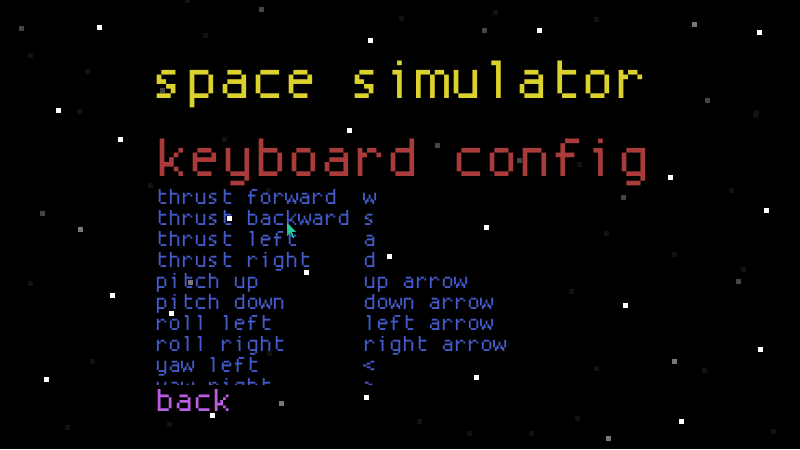
\includegraphics[scale=0.5]{../images/08-keyboard_config.png}
  \caption{Keyboard config.  User may set the button by pressing the desired key.}
\end{figure}

\begin{figure}[H]
  \centering
  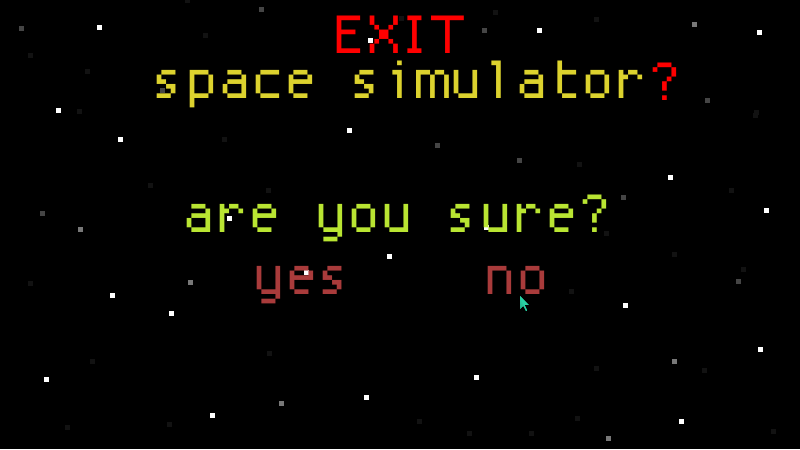
\includegraphics[scale=0.5]{../images/09-exit.png}
  \caption{Exit screen confirms the player's desire to exit the program.}
\end{figure}

\begin{figure}[H]
  \centering
  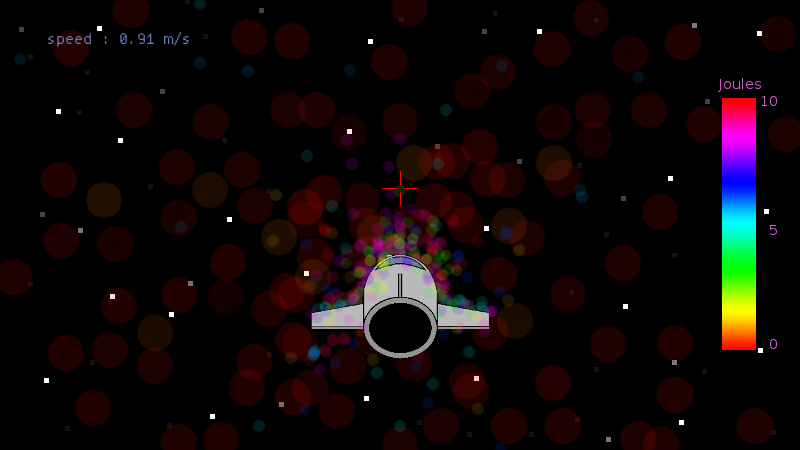
\includegraphics[scale=0.5]{../images/10-nebula.png}
  \caption{Here we have the spacecraft flying into the nebula, with a colorbar to show the energy level of the nebula particles.  The red `X' in the middle is a crosshair used for guiding the ship and firing rockets when implemented.  The speed of the craft is shown in the top left corner.  Notice that the color of the nebula changes as the craft pushes nebula gas particles out of its path.}
\end{figure}

\begin{figure}[H]
  \centering
  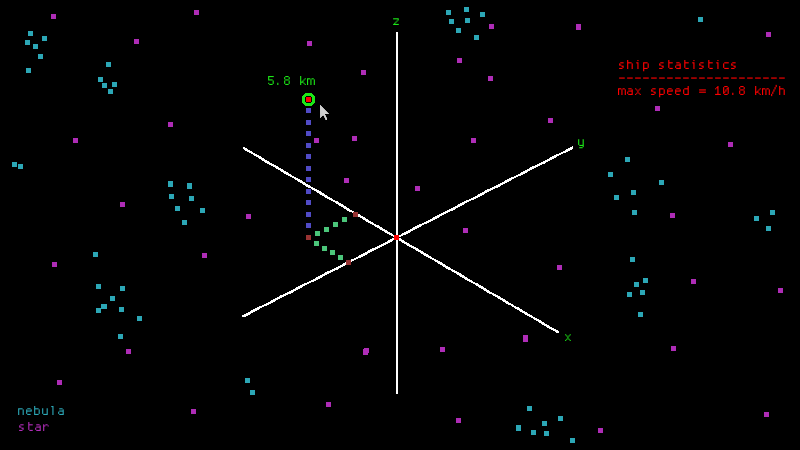
\includegraphics[scale=0.5]{../images/11-map.png}
  \caption{Map screen - the player selects a planet (purple) or a nebula (blue) to see the distance to it.  The ship is located at the red dot in the intersection of the axes.  Once a destination is clicked, the green circle appears around the planet.  This green circle will remain in the flight screen as well to enable the player to navigate to their chosen destination.  The view may be rotated by depressing the right mouse button and dragging the mouse up and down, left and right.  Extra ship statistics are also shown to the left of the screen, here with only the max attainable speed of the craft.}
\end{figure}

\begin{figure}[H]
  \centering
  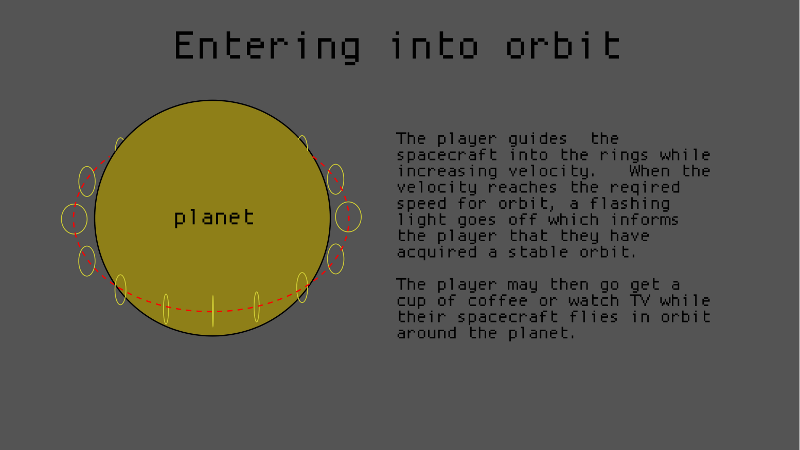
\includegraphics[scale=0.5]{../images/12-orbit.png}
  \caption{Concept for entering the spacecraft into orbit.}
\end{figure}


\end{document}


